\subsection{System Response to Internal Conditions}
What is this? We never covered zero-input response in 330.

\subsection{The Unit Impulse Response}
The book goes right into describing systems as dif. eq's. Is this the approach we want to have as well? I know before we broke down systems into a few ways: Convolution, difference equations, dif. eq, and laplace?

I personally find a complete and full derivation of something such as convolution actually helps me in my understanding and intuition. When the math is abstracted it feels like theres gaps in my understanding and like I'm missing why something is something.

The below figure demonstrates a pretty good visualization for what convolution really does. I think this was never made clear (for me) in the videos.

I want to redo the convodemo from 203 with a better GUI and make a version for continuous convolution.

I never knew until now that convolution with the unit impulse is just the function $x(t)$ itself.

The book itself has lots of good matlab examples.

What is the thought process of discrete vs continuous for teaching order? Currently 330 splits it up in terms of "operation". It first goes over convolution and then difference and differential equations. The book groups everything in terms of continuous or discrete instead.

What is easier to intuitively understand first, discrete or continuous?

Again, I really like how they format this.
\begin{itemize}
    \item Introduction
    \item Theory
    \item Example
    \item Matlab!!!
\end{itemize}

\begin{figure}
    \center 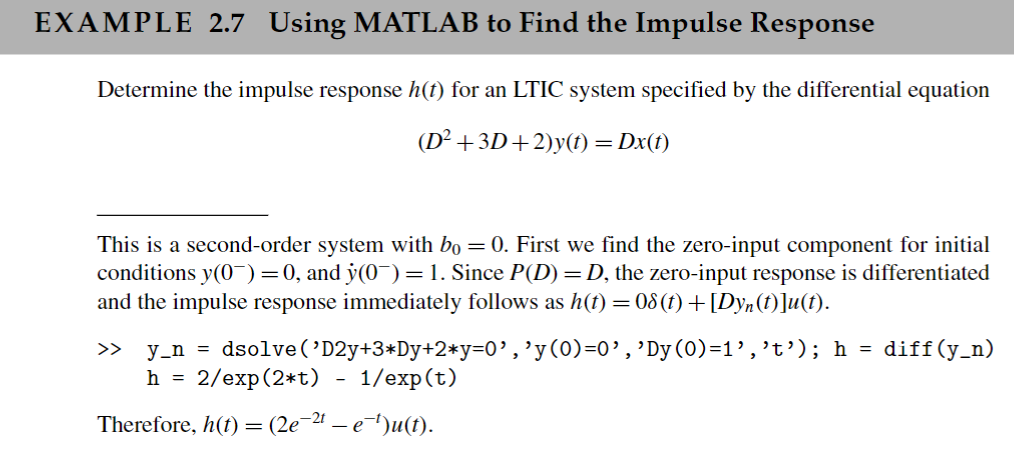
\includegraphics[width = 0.75\textwidth]{images/example 2.7.png}
\end{figure}

\begin{figure}
    \begin{center}
        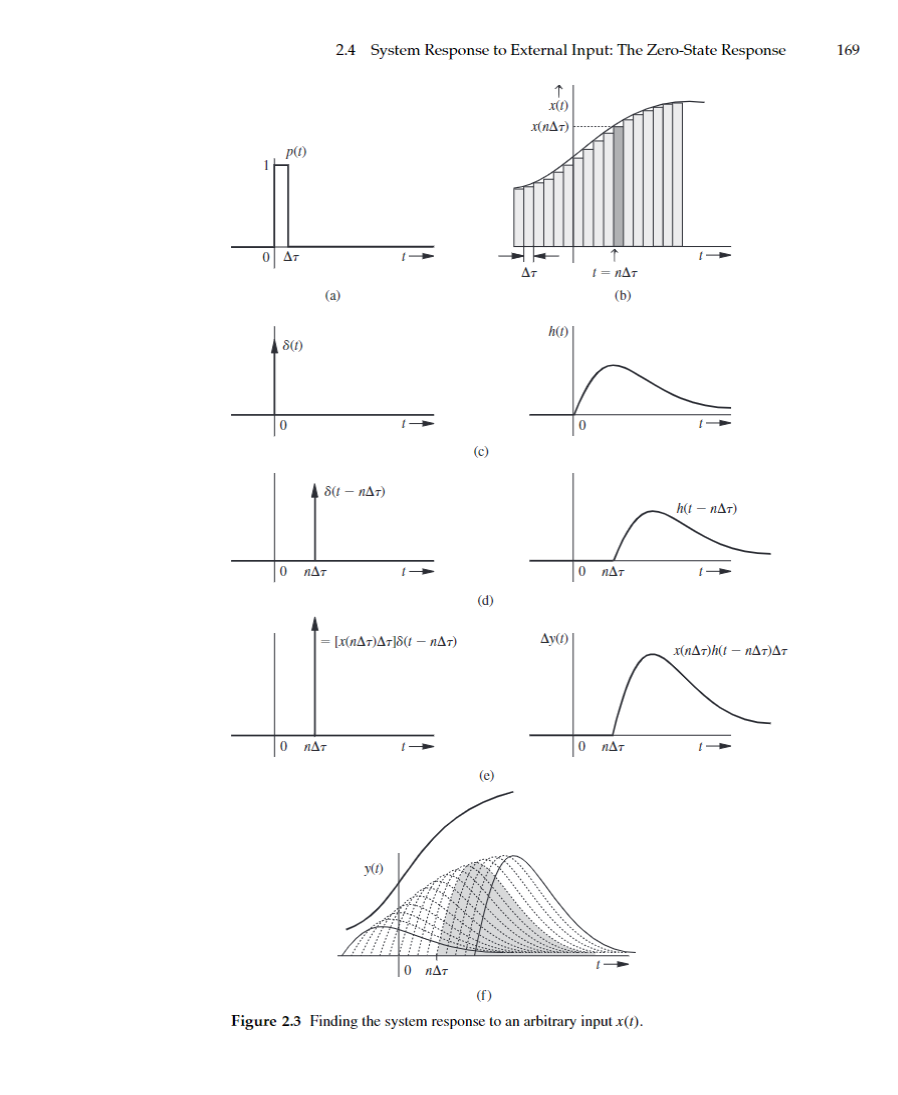
\includegraphics[width = 0.75\textwidth]{images/convolution.png}
    \end{center}
\end{figure}

\begin{figure}
    \begin{center}
       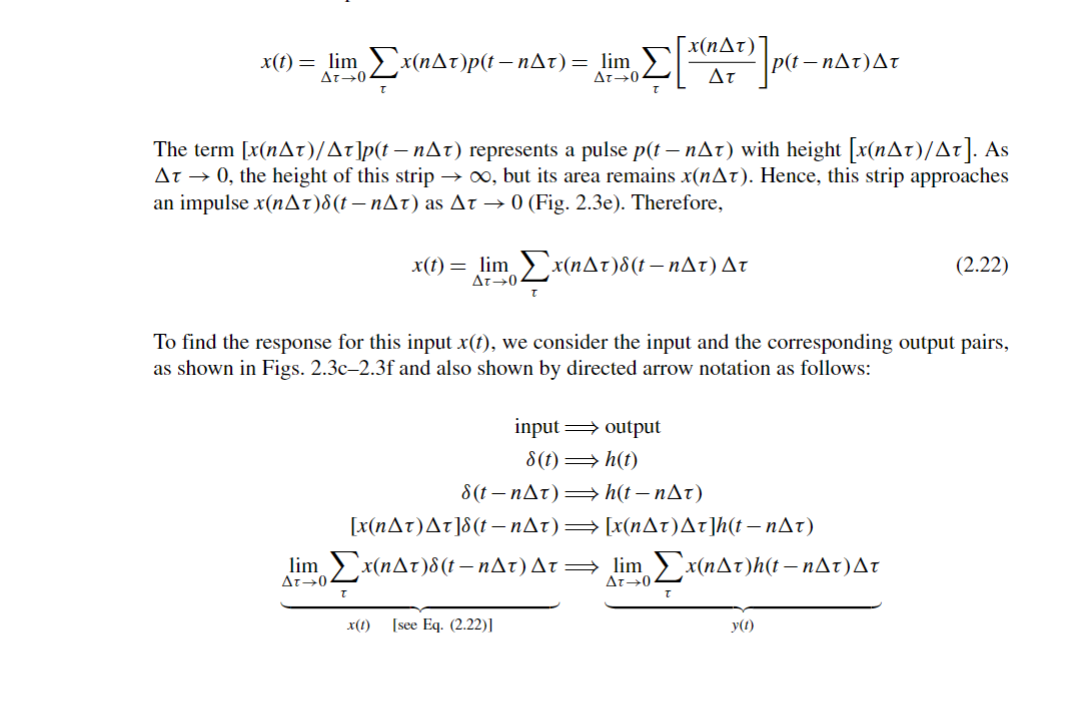
\includegraphics[width = 0.75\textwidth]{images/convolution_deriv.png}
    \end{center}
\end{figure}

\textbf{NOTE: Pg 189-190 has a good intuitive explanation of system response.}

\subsection{2.7-1 Op Amp Script Example}

KCL equation at +v(t) node
\[\frac{x(t) - v(t)}{R_3} + \frac{y(t) - v(t)}{R_2} + \frac{0-v(t)}{R_1} - C_2\odv{v}{t} = 0\]

KCL equation at inverting pin
\[\frac{v(t)}{R_1} + C_1\odv{y}{t}\]

\begin{example}
    \center
    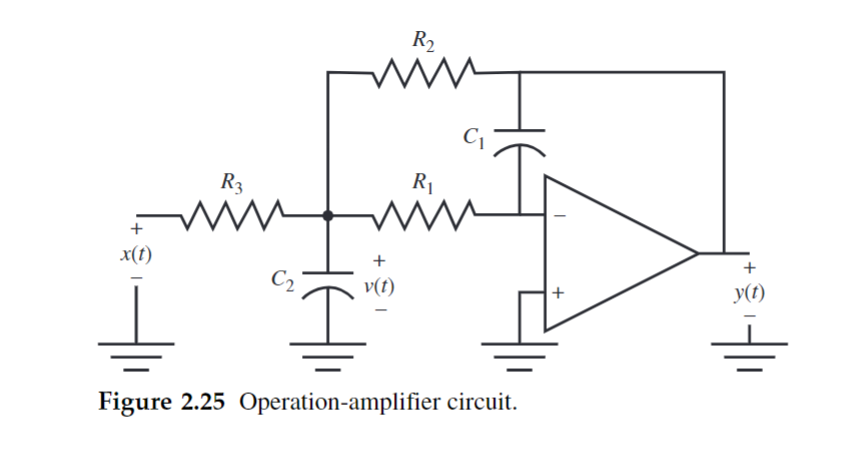
\includegraphics{images/op amp circuit.png}
\end{example}

Characteristic equation:
\[\lambda^2 + \frac{1}{C_2}{\frac{1}{R_1 + R_2 + R_3}}\lambda + \frac{1}{R_1R_2C_1C_2} = (a_0\lambda^2 + a_1\lambda + a_2) = 0\]



